\documentclass[a4paper, 12pt]{article}        % General format
%\documentclass[a4paper, 14pt]{extarticle}    % Advanced format

%%%% Charset
\usepackage{cmap}                             % Make PDF files searchable and copyable
\usepackage[utf8x]{inputenc}                  % Accept different input encodings
\usepackage[T2A]{fontenc}                     % Russian font
\usepackage[russian]{babel}                   % Multilingual support (T2A)

%%%% Graphics
\usepackage[dvipsnames]{xcolor}               % Driver-independent color extensions
\usepackage{graphicx}                         % Enhanced support for graphics
\usepackage{wrapfig}                          % Produces figures which text can flow around
\usepackage{float}                            % Improved interface for floating objects

%%%% Graphs
\usepackage{tikz}                             % Creating graphics programmatically
\usetikzlibrary{arrows}                       % Arrows for tikz

%%%% Math
\usepackage{amsmath}                          % American Mathematical Society (AMS) math facilities
\usepackage{amsfonts}                         % fonts from the AMS
\usepackage{amssymb}                          % additional math symbols

%%%% Typography (don't forget about cm-super)
\usepackage{microtype}                        % subliminal refinements towards typographical perfection
\linespread{1.3}                              % line spacing
\usepackage[left=2.5cm, right=1.5cm, top=2.5cm, bottom=2.5cm]{geometry}
\setlength{\parindent}{0pt}                   % we don't want any paragraph indentation
\usepackage{parskip}                          % add distance between paragraphs

%%%% Tables
\usepackage{tabularx}                         % Enhanced tables
\usepackage{multirow}                         % For tabular
\usepackage{hhline}                           % For tabular

%%%% Other
\usepackage{url}                              % Verbatim with URL-sensitive line breaks
\usepackage{fancyvrb}                         % Sophisticated verbatim text
\setcounter{secnumdepth}{5}                   % Turn on subsection numbering

%------------------------------------------------------------------------------
\usepackage{listings}                         % typeset source code listings

% The colors for syntax highlighting.
\definecolor{mygreen}{HTML}{3F7F5F}           % color values Red, Green, Blue
\definecolor{mylilas}{RGB}{170,55,241}

% Code listing settings
\lstset{language=Matlab,%
    %basicstyle=\color{red},
    breaklines    =  true,                    % wrap long lines
    morekeywords  =  {matlab2tikz},           %
    keywordstyle  =  \color{blue},            %
    morekeywords  =  [2]{1},                  %
    keywordstyle  =  [2]{\color{black}},      %
    identifierstyle= \color{black},           %
    stringstyle   =  \color{mylilas},         %
    commentstyle  =  \color{mygreen},         %
    showstringspaces=false,                   % don't mark spaces in strings
    frame         =  tblr                     % draw a frame at all sides of the code block
    rulecolor     =  \color{frame},           % frame color
    tabsize       =  2,                       % tab space width
    showstringspaces=false,                   % don't mark spaces in strings
    numbers       =  left,                    %
    numberstyle   =  {\tiny \color{black}},   % size of the numbers
    numbersep     =  9pt,                     % this defines how far the numbers are from the text
    emph          =  [1]{for,end,break},      %
    emphstyle     =  [1]\color{red},          % some words to emphasise
    %emph         =  [2]{word1,word2},        %
    %emphstyle    =  [2]{style},              %
    extendedchars =  true,                    % For the Russian language support
    literate=
        {Ö}{{\"O}}1                    {Ä}{{\"A}}1                    {Ü}{{\"U}}1
        {ß}{{\ss}}1                    {ü}{{\"u}}1                    {ä}{{\"a}}1
        {ö}{{\"o}}1                    {~}{{\textasciitilde}}1        {а}{{\selectfont\char224}}1
        {б}{{\selectfont\char225}}1    {в}{{\selectfont\char226}}1    {г}{{\selectfont\char227}}1
        {д}{{\selectfont\char228}}1    {е}{{\selectfont\char229}}1    {ё}{{\"e}}1
        {ж}{{\selectfont\char230}}1    {з}{{\selectfont\char231}}1    {и}{{\selectfont\char232}}1
        {й}{{\selectfont\char233}}1    {к}{{\selectfont\char234}}1    {л}{{\selectfont\char235}}1
        {м}{{\selectfont\char236}}1    {н}{{\selectfont\char237}}1    {о}{{\selectfont\char238}}1
        {п}{{\selectfont\char239}}1    {р}{{\selectfont\char240}}1    {с}{{\selectfont\char241}}1
        {т}{{\selectfont\char242}}1    {у}{{\selectfont\char243}}1    {ф}{{\selectfont\char244}}1
        {х}{{\selectfont\char245}}1    {ц}{{\selectfont\char246}}1    {ч}{{\selectfont\char247}}1
        {ш}{{\selectfont\char248}}1    {щ}{{\selectfont\char249}}1    {ъ}{{\selectfont\char250}}1
        {ы}{{\selectfont\char251}}1    {ь}{{\selectfont\char252}}1    {э}{{\selectfont\char253}}1
        {ю}{{\selectfont\char254}}1    {я}{{\selectfont\char255}}1    {А}{{\selectfont\char192}}1
        {Б}{{\selectfont\char193}}1    {В}{{\selectfont\char194}}1    {Г}{{\selectfont\char195}}1
        {Д}{{\selectfont\char196}}1    {Е}{{\selectfont\char197}}1    {Ё}{{\"E}}1
        {Ж}{{\selectfont\char198}}1    {З}{{\selectfont\char199}}1    {И}{{\selectfont\char200}}1
        {Й}{{\selectfont\char201}}1    {К}{{\selectfont\char202}}1    {Л}{{\selectfont\char203}}1
        {М}{{\selectfont\char204}}1    {Н}{{\selectfont\char205}}1    {О}{{\selectfont\char206}}1
        {П}{{\selectfont\char207}}1    {Р}{{\selectfont\char208}}1    {С}{{\selectfont\char209}}1
        {Т}{{\selectfont\char210}}1    {У}{{\selectfont\char211}}1    {Ф}{{\selectfont\char212}}1
        {Х}{{\selectfont\char213}}1    {Ц}{{\selectfont\char214}}1    {Ч}{{\selectfont\char215}}1
        {Ш}{{\selectfont\char216}}1    {Щ}{{\selectfont\char217}}1    {Ъ}{{\selectfont\char218}}1
        {Ы}{{\selectfont\char219}}1    {Ь}{{\selectfont\char220}}1    {Э}{{\selectfont\char221}}1
        {Ю}{{\selectfont\char222}}1    {Я}{{\selectfont\char223}}1    {і}{{\selectfont\char105}}1
        {ї}{{\selectfont\char168}}1    {є}{{\selectfont\char185}}1    {ґ}{{\selectfont\char160}}1
        {І}{{\selectfont\char73}}1     {Ї}{{\selectfont\char136}}1    {Є}{{\selectfont\char153}}1
        {Ґ}{{\selectfont\char128}}1
}

\usepackage{caption}                          % Set listing header
\DeclareCaptionFont{white}{\color{сaptiontext}}
\DeclareCaptionFormat{listing}{\parbox{\linewidth}{\colorbox{сaptionbk}{\parbox{\linewidth}{#1#2#3}}\vskip-4pt}}
%\captionsetup[lstlisting]{format=listing,labelfont=white,textfont=white}
%\renewcommand{\lstlistingname}{Листинг}       % Renaming 'Listings' in the right structure name
%------------------------------------------------------------------------------

\begin{document}

%------------------------------------------------
\begin{titlepage}
\thispagestyle{empty}

\begin{center}
Санкт-Петербургский политехнический университет Петра Великого\\
Институт Информационных Технологий и Управления \\*
Кафедра компьютерных систем и программных технологий \\*
\hrulefill
\end{center}

\vspace{15em}

\begin{center}
\Large Отчёт по практической работе\\по предмету «Системное программное обеспечение» \\
\end{center}

\vspace{1em}

% \linebreak
\begin{center}
\textsc{\textbf{Процесс загрузки операционной системы Linux}}
\end{center}

\vspace{20em}

\begin{flushleft}
Работу выполнил студент гр. 53501/3 \hrulefill Мартынов С. А. \\
\vspace{1.5em}
Работу принял преподаватель \hrulefill Душутина Е. В. \\
\end{flushleft}

\vspace{\fill}

\begin{center}
Санкт-Петербург \\
2015
\end{center}

\end{titlepage}
%------------------------------------------------
\setcounter{page}{2} % Титульная страница
\tableofcontents

%------------------------------------------------------------------------------

\newpage
\section*{Постановка задачи}
\addcontentsline{toc}{section}{Постановка задачи}

\vspace{2em}

В рамках данной работы необходимо ознакомиться приниципами написания драйверов и реализовать драйвер сетевого устройства.

\vspace{1em}

Привести краткую информация о контроллере сетевого устройства и его технические характеристики. Дать описание порядка разработки драйвера и способы взаимодействия ядра с апараторуй. Для используемых структур представить назначение основных полей. Описать взаимодействие драйвера, находящегося в пространстве ядра, с приложениями уровня пользователя.

\vspace{1em}

Сетевое устройство (сетевая карта) может быть выбрана студентом самостоятельно.
 % Постановка задачи

\newpage
\section*{Введение}
\addcontentsline{toc}{section}{Введение}

Драйвер устройства -- это низкоуровневая программа, содержащая специфический код для работы с устройством, которая позволяет пользовательским программам (и самой ОС) управлять им стандартным образом.

В современных версиях ядра Linux по умолчанию присутствуют все необходимые драйверы для всех поддерживаемых устройств\cite{Love}. Но для старых версий ядра иногда приходится заниматься бэк-портированием драйверов или даже написанием из с нуля, чтобы обеспечить корректную работу железа.

Все устройства можно разделить на:
\begin{itemize}
\item \textbf{Символьные}. Чтение и запись устройства идет посимвольно. Примеры таких устройств: клавиатура, последовательные порты.
\item \textbf{Блочные}. Чтение и запись устройства возможны только блоками, обычно по 512 или 1024 байта. Пример - жесткий диск.
\item \textbf{Сетевые интерфейсы}. Отличаются тем, что не отображаются на файловую систему, т.е. не имеют соответствующих файлов в директории /dev, поскольку из-за специфики этих устройств работа с сетевыми устройствами как с файлами неэффективна. Пример - сетевая карта (eth0).
\end{itemize}

В распоряжении имеется относительно старая материнская плата ASUS P5B на чипсете Intel P965, со встроенной сетевой картой на основе Realtek RTL8111B, для которой будет разработан драйвер, работающий в старой версии ядра Linux.

Это довольно популярная платформа r8169, для которой открыта спецификация. Ссылка на неё приводится в списке использованных материалов. % Введение

\newpage
\section{Фоновые приложения в Linux}

\subsection{Понятие процесса и демона}

В любой многозадачной системе одновременно может быть запущено много программ, то есть много процессов. В действительности в каждый момент времени выполняется только один процесс. Ядро (по средствам планировщика) выделяет каждому процессу небольшой квант времени и по истечении этого кванта передает управление следующему процессу. Кванты времени, выделяемые каждому процессу, на столько малы, что у пользователя создается иллюзия одновременного выполнения многих процессов. Для организации переключения между процессами по истечении кванта времени, выполняется фиксация и сохранение в памяти состояния программы. Этот снимок содержит информацию о состоянии регистров центрального процессора на момент прерывания программы, указание на то, с какой команды возобновить исполнение программы (состояние счетчика команд), содержимое стека и подобные данные. Когда процесс снова получает в свое распоряжение ЦП, состояние регистров ЦП и стека восстанавливается из сделанного снимка и выполнение программы возобновляется в точности с того места, где она была остановлена. Такие же действия выполняются в тех случаях, когда какому-то процессу необходимо вызвать некоторую системную функцию (вызов ядра)\cite{Cit1}.

Кроме организации переключения процессов, ядро в многозадачной системе отвечает за изоляцию процессов -- два процесса не должны одновременно изменять какие-то данные одном участке памяти. Для этого каждому процессу выделяется свое виртуальное адресное пространство. Его размер может даже превышать размер реальной оперативной памяти, что обеспечивается за счет применения страничной организации памяти и механизма свопинга. И физическая и виртуальная память организована в виде страниц -- областей памяти фиксированного размера (обычно 4 Кбайта). Если страница долго не используется, ее содержимое переносится в область свопинга на жестком диске, а страница в оперативной памяти предоставляется в распоряжение другого процесса. Подсистема управления памятью поддерживает таблицу соответствия между страницами виртуальной памяти процессов и страницами физической памяти (включая страницы, перенесенные в область свопинга). В современных компьютерных системах эти механизмы реализуются на аппаратном уровне с помощью устройств управления памятью -- Memory Management Unit (MMU). Если процесс обращается к странице виртуальной памяти, которая размещается в оперативной памяти, операция чтения или записи осуществляется немедленно. Если же страница в оперативной памяти отсутствует, генерируется аппаратное прерывание, в ответ на которое подсистема управления памятью определяет положение сохраненного содержимого страницы в области свопинга, считывает страницу в оперативную память, корректирует таблицу отображения виртуальных адресов в физические, и сообщает процессу о необходимости повторить операцию. Все эти действия невидимы для приложения, которое работает с виртуальной памятью. При этом один процесс не может прочитать что-либо из памяти (или записать в нее) другого процесса без «разрешения» на то со стороны подсистемы управления памятью. При такой организации работы крах одного процесса никак не повлияет на другие выполняющиеся процессы и на всю систему в целом.

Среди всех процессов можно выделить несколько особых типов процессов.

Системные процессы являются частью ядра и всегда находятся в оперативной памяти. Такие процессы не имеют соответствующих им программ в виде исполняемых файлов и запускаются особым образом при инициализации ядра системы. Примерами системных процессов являются планировщик процессов, диспетчер свопинга, диспетчер буферного кэша, диспетчер памяти ядра. Такие процессы являются фактически потоками ядра.

Демоны отличаются от обычных процессов только тем, что они работают в интерактивном режиме. Если с обычным процессом всегда ассоциирован какой-то терминал или псевдо терминал, через который осуществляется взаимодействие процесса с пользователем, то демон такого терминала не имеет. Демоны обычно используются для выполнения сервисных функций, обслуживания запросов от других процессов, причем не обязательно выполняющихся на данном компьютере. Пользователь не может непосредственно управлять демонами, он может влиять на их работу, только посылая им какие-то задания, например, отправляя документ на печать.

Главным демоном в системе является демон init\cite{Cit2}. Он является прародителем всех процессов в системе и имеет идентификатор 1. Выполнив задачи, поставленные в ему в файле inittab, демон init не завершает свою работу -- он постоянно находится в памяти и отслеживает выполнение других процессов.

Прикладные процессы -- это все остальные процессы, выполняющиеся в системе. Как правило, эти процессы порождаются в рамках сеанса работы пользователя. В каждом таком сеансе работы вначале запускается оболочка (командный интерпретатор) shell. Этот экземпляр оболочки называется login shell и завершение соответствующего процесса приводит к отключению пользователя от системы.

\subsection{Создание демона Linux}

Для задачи демонизации будем использовать программу из предыдущей лабораторной работы. Она будет отслеживать состояние сетевого интерфейса и записывать результаты своей работы в системный журнал. Код демона представлен в листинге 1.

\lstinputlisting[language=C++, caption={Исходный код демона Linux (src/daemons/lin/main.cpp)}]
{../../src/daemons/lin/main.cpp}

Логика работы самого приложения не изменилась, изменился только способ запуска. После проверки аргументов (стр. 19), приложение выполняет операцию fork() (стр. 24), после чего "родительская" часть спокойно завершает свою работу (стр. 59), а "дочернее" выполняет ряд операций, характерных для демона.

Для начала в процессе потомка нужно разрешить выставлять все биты прав на создаваемые файлы, это избавляет от проблемы с правами доступа (стр. 27). Потом создаётся новый сеанс, чтобы не зависеть от родителя (стр. 28). Далее осуществляется переход в корень диска, если этого не сделать, то могут быть проблемы, к примеру с размонтированием дисков (стр. 29). И в конце происходит закрытие дескрипторов ввода/вывода/ошибок, так как демону они не понадобятся (стр. 30-32).

После запуска демона, убедиться в его работоспособности можно так

\begin{Verbatim}[frame=single]
user@host$ ps aux | grep netmonitor 
sam       5776 31.0  0.0  13528   180 ?        Ss   21:25   0:13 ./netmonitor enp2s0
user@host$
\end{Verbatim}

\subsection{Работа с системным журналом}

Функция системного журналирования (т.н. "логи" или логирование) -- это основной источник информации о работе системы и ошибках. Журналирование может осуществляться на локальной системе, а так же сообщения журналирования могут пересылаться на удаленную систему. Журналирование осуществляется при помощи демона syslogd или rsyslogd. Журнал обычно получает входную информацию при помощи сокета /dev/log (локально) или с udp-порта 514 (с удаленных машин)\cite{Cit3}.

Соединение с журналом было установлено в строке 18. Первый параметр сообщил системному журналу имя приложения, которое будет использоваться при ведении записей, а два оставшихся поля состоят из флагов флагов\cite{Cit2}.

Предпоследнее поле (option) принимает дизъюнкцию следующих значений:
\begin{itemize}
\item \textbf{LOG\_CONS} написать сообщение об ошибке прямо на консоли, если была ошибка при записи данных в системный журнал; 
\item \textbf{LOG\_NDELAY} устанавливать соединение немедленно (обычно оно устанавливается только при поступлении первого сообщения); 
\item \textbf{LOG\_NOWAIT} не ожидает дочерние процессы которые могут быть созданы во время отправки этого сообщения
\item \textbf{LOG\_ODELAY}обратно от LOG\_NDELAY; открытие соединения откладывается до вызова syslog(). 
\item \textbf{LOG\_PERROR} посылать сообщение еще и в поток stderr; 
\item \textbf{LOG\_PID} добавлять к каждому сообщению идентификатор 
\end{itemize}

Последнее поле (facility) используется для указания типа программы, записывающей сообщения и принимает дизъюнкцию следующих значений:
\begin{itemize}
\item \textbf{LOG\_AUTH} сообщения о безопасности/авторизации (РЕКОМЕНДУЕТСЯ использовать вместо него LOG\_AUTHPRIV). 
\item \textbf{LOG\_AUTHPRIV} сообщения о безопасности/авторизации (частные); 
\item \textbf{LOG\_CRON} демон часов (cron и at); 
\item \textbf{LOG\_DAEMON} другие системные демоны; 
\item \textbf{LOG\_KERN} сообщения ядра; 
\item \textbf{LOG\_LOCAL0 до LOG\_LOCAL7} зарезервированы для определения пользователем; 
\item \textbf{LOG\_LOG\_LPR} подсистема принтера; 
\item \textbf{LOG\_MAIL} почтовая подсистема; 
\item \textbf{LOG\_NEWS} подсистема новостей USENET; 
\item \textbf{LOG\_SYSLOG} сообщения, генерируемые syslogd; 
\item \textbf{LOG\_USER} (по умолчанию) -- общие сообщения на уровне пользователя;
\item \textbf{LOG\_UUCP} -- подсистема UUCP 
\end{itemize}

При записи сообщения, можно указать его тип (критичность) для последующей фильтрации (показывать сообщения не ниже определённого уровня). Это используется в строках 20, 42, 46, 56, 60.

Уровень важности сообщения по понижению:

\begin{itemize}
\item \textbf{LOG\_EMERG} система остановлена; 
\item \textbf{LOG\_ALERT} требуется немедленное вмешательство; 
\item \textbf{LOG\_CRIT} критические условия; 
\item \textbf{LOG\_ERR} ошибки; 
\item \textbf{LOG\_WARNING} предупреждения; 
\item \textbf{LOG\_NOTICE} важные рабочие условия; 
\item \textbf{LOG\_INFO} информационные сообщения; 
\item \textbf{LOG\_DEBUG} сообщения об отладке.
\end{itemize}

В строке 64 соединение с системным логом закрывается.

Записи системного лога попадают в файл /var/log/syslog. В листинге 2 показан вывод (без форматирования) некоторых (10 последних) строк этого файла. Важно отметить, что когда системный журнал получает повторяющиеся события (т.е. состояние счётчиков на сетевой карте не успело измениться), он делает пометку о повторе, вместо прямого дублирования.

\lstinputlisting[language={},caption={Системный журнал Linux}]{res/syslog.output}
 % Фоновые приложения в Linux

\newpage
\section{Дистрибуция пакетов в Linux}

Программное обеспечение в ОС Ubuntu Linux распространяется в так называемых deb-пакетах. Обычно при установке программы из репозитория система автоматически скачивает и устанавливает deb-пакеты. Главной причиной использовать этот путь является автоматическое разрешение зависимостей. Программу можно установить, только если уже установлены пакеты, от которых она зависит. Такая схема позволяет избежать дублирования данных в пакетах (например, если несколько программ зависят от одной и той же библиотеки, то не придётся пихать эту библиотеку в пакет каждой программы -- она поставится один раз отдельным пакетом). В отличие от, например, Slackware или Windows, в Ubuntu зависимости разрешаются пакетным менеджером (Synaptic, apt, Центр приложений, apt-get, aptitude) -- он автоматически установит зависимости из репозитория. Зависимости придётся устанавливать вручную, если нужный репозиторий не подключен, недоступен, если нужного пакета нет в репозитории, если вы ставите пакеты без использования пакетного менеджера (используете Gdebi или dpkg), если вы устанавливаете программу не из пакета (компилируете из исходников, запускаете установочный run/sh скрипт). Операционные системы на базе Debian распространяют пакеты deb, на базе RedHat -- rpm.

\subsection{Создание DEB/RPM/TGZ пакетов}

CheckInstall -- это удобная утилита, позволяющая создавать бинарные пакеты для Linux из исходного кода приложения. После компиляции программного обеспечения checkinstall может автоматически сгенерировать Slackware-, RPM- или Debian-совместимый пакет, который впоследствии может быть полностью удалён через соответствующий менеджер пакетов. Эта возможность является предпочтительной при установке любых пакетов\cite{Cit4}.

\textbf{Установка программы checkinstall}

Установка пакета checkinstall не должна вызвать особых сложностей. В операционных системах, использующих DEB пакеты, установка производится командой:

\begin{Verbatim}[frame=single]
user@host$ sudo apt-get install checkinstall
\end{Verbatim}

В операционной системе, использующей RPM пакеты, установка пакета checkinstall выполняется командой:

\begin{Verbatim}[frame=single]
user@host$ sudo rpm -i checkinstall
\end{Verbatim}

Если такой пакет в Вашей ОС не обнаружен, то следует посетить домашнюю страницу проекта и скачать требуемую версию для Вашего дистрибутива:

\url{http://checkinstall.izto.org/download.php}

\textbf{Компилирование исходников}

Далее следует перейти в каталог с программой и провести её компиляцию.

Программа, которая была рассмотрена в предыдущем разделе может быть собрана следующим образом.

\begin{Verbatim}[frame=single]
user@host$ g++ --std=c++14 main.cpp -o netmonitor
\end{Verbatim}

\textbf{Создание DEB-пакета из исходного кода}

Программа checkinstall создает и устанавливает пакет для основных ОС. Тип пакета (DEB или RPM) checkinstall определяет сам. Для жесткого указания типа создаваемого пакета используем команду checkinstall с ключами:

Создает и устанавливает RPM пакет

\begin{Verbatim}[frame=single]
user@host$ sudo checkinstall -R
\end{Verbatim}

Создает и устанавливает DEB пакет
\begin{Verbatim}[frame=single]
user@host$ sudo checkinstall -D
\end{Verbatim}

Создает и устанавливает TGZ пакет (дистрибутивы: Slackware, Zenwalk, DeepStyle, Vektorlinux, Mops)
\begin{Verbatim}[frame=single]
user@host$ sudo checkinstall -S
\end{Verbatim}

Далее следует ответить на несколько вопросов. По умолчанию все ответы на задаваемые вопросы подходят в большинстве случаев, поэтому везде нажимаем Enter.

\subsection{Создание PKGBUILD}

Пользовательский репозиторий Arch Linux (Arch User Repository, AUR) -- это поддерживаемое сообществом хранилище ПО для пользователей Arch. Он содержит описания пакетов (файлы PKGBUILD), которые позволят скомпилировать пакет из исходников с помощью makepkg и затем установить его, используя pacman. В AUR пользователи могут добавлять свои собственные сборки пакетов (PKGBUILD и другие необходимые файлы). Сообществу предоставлена возможность голосовать за эти пакеты или против них. Если пакет становится популярным, распространяется под подходящей лицензией и может быть собран без дополнительных сложностей, то, вероятно, он будет перенесен в репозиторий community (непосредственно доступный при помощи утилит pacman и abs)\cite{Cit4}.

Файл PKGBUILD по сути напоминает Makefile, и требует установки значений следующих переменных в зависимости от пакета:

\begin{itemize}
\item pkgname -- название пакета. Можно использовать только строчные английские буквы. Значение этой переменной большой роли не играет, но может помочь, если установить сюда имя рабочей директории, или, например, имя файла с исходным кодом (*.tar.gz), который требуется загрузить
\item pkgver -- версия пакета. Эта переменная может содержать буквы, цифры, знаки препинания, но не может содержать дефисов. Содержимое этой переменной зависит от метода присвоения версий (major.minor.bugfix, major.date, и т.д.) который использует программа. Чтобы следующие шаги были наиболее эффективными и лёгкими, рекомендуется включить номер версии в имя файла с исходным кодом. 
\item pkgrel -- число, которое нужно увеличивать каждый раз после новой сборки пакета. При первой сборке пакета значение pkgrel должно быть установлено в "1". Цель этой переменной состоит в том, чтобы различать разные сборки пакета одной и той же версии.
\item pkgdesc -- краткое описание пакета, обычно не более 76 символов.
\item arch -- список архитектур, где может быть использован данный PKGBUILD (обычно это "i686"). 
\item url -- адрес веб-сайта программы, где заинтересовавшиеся могут получить более подробную информацию о программе.
\item license -- тип лицензии (может быть 'unknown').
\item depends -- список пакетов, разделенный пробелами, которые должны быть установлены до использования пакета. Во избежании проблем, имена пакетов заключаются в апострофы ('), а весь массив в скобки. Используя математическое "больше или равно", можно указать минимальную допустимую версию пакета-зависимости.
\item makedepends -- список пакетов, которые потребуются для сборки пакета, но которые не нужны для его использования.
\item provides -- список пакетов, необходимость в которых пропадает, так как собираемый пакет выполняет, по крайней мере, похожие функции.
\item conflicts -- список пакетов, которые, если установлены, могут создать проблемы во время использования собираемого пакета.
\item replaces -- список пакетов, которые заменит собираемый пакет.
\item source -- список файлов, которые потребуются во время сборки пакета. Здесь должна быть ссылка на архив с исходным кодом программы (в большинстве случаев такая ссылка представляет из себя HTTP или FTP ссылку, заключённую в кавычки).
\item md5sums -- список контрольных сумм для файлов из предыдущей переменной, разделенных пробелами и заключённых в апострофы. Как только станут доступны все файлы из списка source, md5 суммы файлов будут автоматически сгенерированы и проверены на соответствие с этим списком.
\end{itemize} % Дистрибуция пакетов в Linux

\newpage
\section{Фоновые приложения в Windows}

\subsection{Службы Windows}

Служба (сервис от англ. service) - это программы, которые автоматически запускаются системой при загрузке Windows и выполняются в любом случае, вне зависимости от действий пользователя.

В большинстве случаев службам запрещено взаимодействие с консолью или рабочим столом пользователей (как локальных, так и удалённых), однако для некоторых сервисов возможно исключение — взаимодействие с консолью (сессией с номером 0, в которой зарегистрирован пользователь локально или при запуске службы mstsc с ключом /console).

Существует четыре режима для сервисов:
\begin{itemize}
\item запрещён к запуску;
\item ручной запуск (по запросу);
\item автоматический запуск при загрузке компьютера;
\item обязательный сервис (автоматический запуск и невозможность (для пользователя) остановить сервис).
\end{itemize}

Windows предлагает программу Service Control Manager, с её помощью можно управлять созданием, удалением, запуском и остановкой служб. Приложение, имеющее статус сервиса, должно быть написано таким образом, чтобы оно могло принимать сообщения от Service Control Manager. Затем, одним или несколькими вызовами API, имя службы и другие атрибуты, такие, как его описание, регистрируются в Service Control Manager.

Список служб находится в ветке реестра HKEY\_LOCAL\_MACHINE\textbackslash SYSTEM\textbackslash CurrentControlSet\textbackslash Services. Значения параметра «Start» имеют тип «REG\_DWORD» и могут принимать значения: «0», «1», «2», «3» и «4» (когда служба не запускается, то есть запуск данной службы запрещен)\cite{Cit5}.

Сервисы Windows по умолчанию запускаются от имени пользователя «LocalSystem», который обладает полными правами в системе (превосходящими права даже учётной записи Administrator). Рабочим каталогом будет системный каталог Windows (обычно C:\textbackslash WINNT или C:\textbackslash WINDOWS), а каталог для хранения временных файлов будет C:\textbackslash WINNT\textbackslash TEMP.

Поскольку это не настоящий пользователь, а «виртуальный», появляются некоторые трудности, когда приложению необходимо сохранить данные, относящиеся к пользователю (user-specific data), поскольку не существует папки этого пользователя.

Важно также то, что в случае если служба работает от имени локального пользователя (реальный пользователь созданный для служебных целей) если пароль такого пользователя изменён, сервис не будет запускаться до тех пор, пока пароль для сервиса тоже не будет изменен.

\subsection{Создание службы Windows с помощью программы Sc.exe}

Этот способ является рекомендованным корпорацией Microsoft\cite{Cit6}.

Для создания служб Windows можно использовать программу Sc.exe, включенную в пакет ресурсов Resource Kit, которая реализует вызовы ко всем функциям интерфейса прикладного программирования (API) управления службами Windows. Настроить параметры для этих функций можно, задав их в командной строке. С помощью средства Sc.exe имеется возможность запросить состояние службы и получить значения, хранящиеся в полях структуры состояний. SC позволяет задавать имя удаленного компьютера, что дает возможность вызвать функции интерфейса API службы и посмотреть структуры состояния службы на удаленном компьютере.

Кроме того, Sc.exe позволяет вызвать любую функцию интерфейса API управления службами и изменить любой параметр, используя командную строку. Данное средство предоставляет удобный способ создания и изменения записей службы в реестре и в базе данных диспетчера служб. Для настройки службы нет необходимости вручную создавать записи в реестре и затем перезагружать компьютер, чтобы обеспечить обновление базы данных диспетчером служб.

Программа Sc.exe использует следующий синтаксис:

\begin{Verbatim}[frame=single]
sc [Servername] Command Servicename
\end{Verbatim}

Команда \textbf{sc create} создает запись службы в реестре и в базе данных диспетчера служб.

Синтаксис
\begin{Verbatim}[frame=single]
sc [Servername] create Servicename [Optionname=Optionvalue...
\end{Verbatim}

Параметры могут быть следующими:
\begin{itemize}
\item Servername -- необязательный параметр. Задает имя удаленного сервера, на котором будут запускаться команды.
\item Command -- задает команду sc. Команды могут быть следующие:
\begin{itemize}
\item Config -- изменяет конфигурацию службы (постоянные параметры).
\item Continue -- посылает службе запрос Continue.
\item Control -- посылает службе запрос Control.
\item Create -- создает службу (добавляет ее в реестр).
\item Delete -- удаляет службу (из реестра).
\item EnumDepend -- перечисляет зависимости служб.
\item GetDisplayName -- указывает отображаемое имя службы.
\item GetKeyName -- указывает имя раздела службы.
\item Interrogate -- посылает службе запрос Interrogate.
\item Pause -- посылает службе запрос Pause.
\item qc -- запрашивает конфигурацию службы.
\item Query -- запрашивает состояние службы или указывает состояние по типам служб.
\item Start -- запускает службу.
\item Stop -- посылает службе запрос Stop.
\end{itemize}
\item Servicename -- указывает имя, присвоенное разделу службы в реестре.
\item Optionname -- служит для указания имен и значений дополнительных параметров.
\item Optionvalue -- задает значение параметра, которому присвоено имя параметром «Optionname».
\end{itemize}

Для выполнения ряда команд необходимо иметь права администратора. Следовательно, необходимо обладать правами администратора на компьютере, на котором создается служба.

Запустим netmonitor в качестве сервиса

\begin{Verbatim}[frame=single]
Sc create MyService binPath=C:\netmonitor.exe DisplayName=″My New Service″ type=own start=auto
\end{Verbatim}

По умолчанию создается служба типа WIN32\_SHARE\_PROCESS с типом запуска SERVICE\_DEMAND\_START. Она не имеет никаких зависимостей и выполняется в контексте безопасности LocalSystem.

Результат добавления приложения в список сервисов показан на рисунке 1.

\begin{figure}[H]
 \centering
 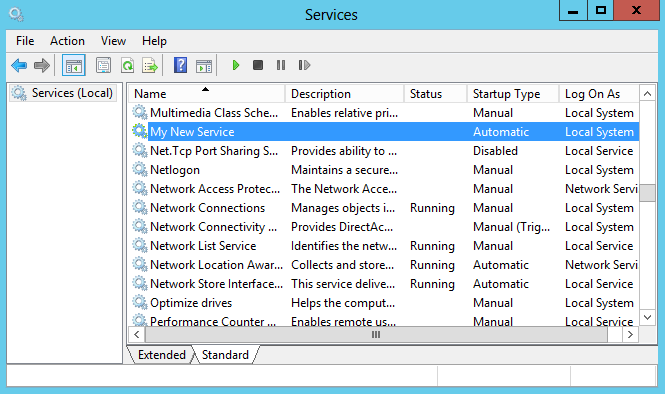
\includegraphics[scale=1]{res/pic001}
 \caption{Добавление сервиса из приложения в windows}
\end{figure}

\subsection{Создание службы Windows с помощью PowerShell}

Возможности управления системой из консоли в последних версиях Windows были значительно расширены. В том числе стало доступно и управление службами Windows. Создать новую службу можно с помощью командлета New-Service. Создадим такой же сервис, как и в предыдущем примере, только добавим к нему описание (Description):

\begin{Verbatim}[frame=single]
New-Service -Name MyService -BinaryPathName C:\netmonitor.exe`
-DisplayName ″My New Service″ -Description ″Very Important Service !!!″
\end{Verbatim}

Изменить параметры службы можно командлетом Set-Service:

\begin{Verbatim}[frame=single]
Set-Service -Name MyService -Description ″Not Very Important Service″ -StartupType Manual
\end{Verbatim}

PowerShell имеет примерно такой же функционал как и Sc.exe. Его особенностью является добавление описаний, но он не имеет простого способа удаления сервисов.

\subsection{Работа с системным журналом Windows}

Взаимодействие с системным журналом в Windows несколько сложнее, чем в Linux. Для начала требуется создать манифест (mc-файл) с описанием сообщений (листинг 2)\cite{Cit7}.

\lstinputlisting[language={},caption={mc-файл с описанием сообщений(src/daemons/win/eventlog.mc)}]{../../src/daemons/win/eventlog.mc}

Следующие две команды генерируют ресурсный файл и хедер для общения с этим ресурсным файлом.

\begin{Verbatim}[frame=single]
mc.exe -A -b -c -h . -r resources eventlog.mc
rc.exe -foresources/eventlog.res resources/eventlog.rc
\end{Verbatim}

После этого остаётся добавить eventlog.res при линковке бинарника, а eventlog.h подключить к основному модулю программы. Использование API системного лога Windows показано в листинге 3.

\lstinputlisting[language=C++, caption={Исходный код службы Windows, демонстрирующий API системного журнала (src/daemons/win/main.cpp)}]
{../../src/daemons/win/main.cpp} % Фоновые приложения в Windows

\newpage
\section{Дистрибуция пакетов в Windows}

В мире Windows распространение программ осуществляется при помощи инсталляционных пакетов.

Inno Setup -- система создания инсталляторов для Windows программ с открытым исходным кодом. Впервые выпущенный в 1997 году, отличается функциональности и стабильности. Кроме того, обладает интерфейсом, к которому привыкли многие пользователи.

Inno Setup графическим интерфейсом, который (по средствам мастера) позволяет создать скрипт, на основании которого генерируется установочный пакет. Скрипт для разрабатываемой программы netmonitor представлен в листинге 5.

\lstinputlisting[language={},caption={Скрипт генерации установочного файла}]{res/netmonitor.iss}

Получив установочный пакет, можно его распространять на других Windows-системах. Установка также происходит при помощи графического мастера и не должна вызывать сложности у пользователя (Рисунок 2).

\begin{figure}[H]
 \centering
 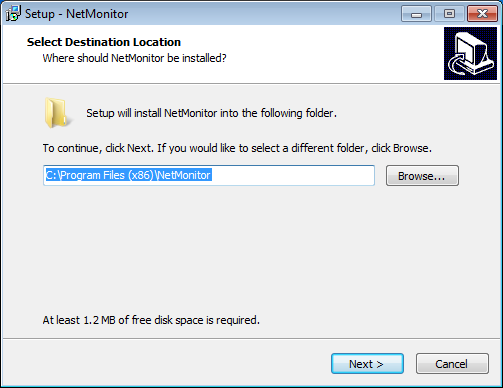
\includegraphics[scale=1]{res/pic002}
 \caption{Интерфейс установки приложения netmonitor}
\end{figure} % Дистрибуция пакетов в Windows

\newpage
%------------------------------------------------
\section*{Заключение}
\addcontentsline{toc}{section}{Заключение}

В данной работе были рассмотрены некоторые системные вызовы, используемые для управления планировщиком при работе с процессами реального времени (POSIX.1b).

В теоретической части было дано описание работы системных вызовов и работы планировщика; по умолчанию все процессы выполняются с интервалос времени равынм 100 мс и приоритетом (nice) 0, который слияет на интервал, позволяя изменять его в диапазоне от 10 мс до 200 мс.

В практической части приведён пример кода, вызывающего изучаемые системные вызовы. Перехват этих вызовов осуществлялся при помощи системной утилиты strace. % Заключение

\newpage
\section*{}
\addcontentsline{toc}{section}{Список литературы}

\begin{thebibliography}{00}

\bibitem{Love} Роберт Лав: «Разработка ядра Linux», Вильямс, 448 стр., 2008, ISBN
5-8459-1085-1, 0-672-32720-1.

\bibitem{Cragon} Harvey G. Cragon: «Computer Architecture and Implementation», Cambridge University Press, 238 pages, 2000, ISBN-10: 521651689.

\bibitem{Rosen} Rami Rosen: «Linux Kernel Networking: Implementation and Theory», Apress, 650 pages, 2014, ISBN-13: 978-1-4302-6196-4.

\bibitem{Realtech} Realtech: RTL8111B, Single-Chip Gigabit LOM Ethernet Controller for PCI Express. Datasheet Rev. 1.4, 02 December 2005, Track ID: JATR-1076-21.

\end{thebibliography} % Источники

%------------------------------------------------------------------------------

\end{document}